\documentclass[utf8]{beamer}
\usepackage{listings}
\usepackage[russian]{babel}
\usetheme{Malmoe}
\title{Архитектура компьютерных сетей}
\author {Компьютерные сети и протоколы}
\date{Лекция 1}
\begin{document}
%--------------------------------------------------------------------------------
\begin{frame}
\titlepage
\end{frame}
%--------------------------------------------------------------------------------
\begin{frame}
\begin{columns}
\column{.5\textwidth}
	\begin{block}{Контактная информация:}
	Андреев~К.~В. ЗАО <<Телум>>
	\begin{description}
		\item [Phone:] +7 (916) 043-07-21
		\item [E-mail:] \url{andreev@telum.ru}
	\end{description}
	\end{block}
\column{.5\textwidth}
	\begin{block}{Основная литература:}
	\centering
	
\includegraphics[width=0.5\textwidth]{pic/tanenbaum.png}
	\newline
	Э.~Таненбаум, Д.~Уэзеролл. ``Компьютерные сети''.
	\newline
	Пятое издание.
	\end{block}
\end{columns}
\end{frame}
%--------------------------------------------------------------------------------
\section{Разнообразие компьютерных сетей и их применение}
\begin{frame}
\frametitle{Необходимость в обмене информацией}
\begin{itemize}
 \item Совместное использование общих ресурсов (клиент-серверная модель)
 \item Передача сообщений и речи (от традиционных телефонных сетей до VoIP и электронной почты)
 \item Распределённые вычисления
 \item Идентификация объектов (RFID -- Radio Frequency Identification)
 \item Системы мониторинга и наблюдения
 \item Системы позиционирования
 \item Профессиональная связь
 \item Электронная коммерция
 \item Поисковые системы (\url{google.com})
 \item \ldots
\end{itemize}
\end{frame}
%--------------------------------------------------------------------------------
\begin{frame}
\frametitle{Варианты использования компьютерных сетей}
Основная функция сетей передачи данных - передача информации на большие расстояния за малое время.
\begin{block}{Классификация сетей по размеру}
\begin{itemize}
 \item Персональные вычислительные сети (Bluetooth, UWB)
 \item Локальные вычислительные сети (Ethernet, WiFi)
 \item Городские сети (WiMAX, PTSN, GSM RAN, 3G UTRAN, 4G E-UTRAN)
 \item Глобальные сети (GSM, UMTS, LTE, SONET, IRIDIUM)
 \item Интернет
\end{itemize}
\end{block}
\begin{block}{Классификация сетей по типу среды передачи}
 Проводные и беспроводные
\end{block}
\end{frame}
%--------------------------------------------------------------------------------
\section{Архитектура сетевого ПО}
%--------------------------------------------------------------------------------
\begin{frame}
\frametitle{Сетевое оборудование и сетевые протоколы}
\begin{itemize}
 \item Разнообразие оборудования
 \item Разнообразие производителей
 \item Разнообразие сред передачи
\end{itemize}
Необходимость структурирования программного обеспечения: использование уровневой архитектуры, точно определённых интерфейсов и иерархии протоколов.
\begin{block}{Уровневая архитектура}
 \begin{itemize}
  \item Реализация некоторого функционала
  \item Скрытие деталей реализации от вышележащих уровней
 \end{itemize}
\end{block}
\begin{block}{Интерфейс}
 Набор примитивных операций, предоставляемых нижнем уровнем верхнему
\end{block}
\end{frame}
%--------------------------------------------------------------------------------
\begin{frame}
\small
\begin{block}{Что значит надёжная передача данных?}
\small
\begin{itemize}
 \item Битовые ошибки в ненадёжных каналах
 \item Ошибки при выборе пути следования данных
 \item Нарушение порядка следования данных
\end{itemize}
\end{block}
\begin{block}{Что значит масштабируемость?}
\small
\begin{itemize}
 \item Вопросы адресации узлов сети
 \item Различные внутренние ограничения различных протоколов
\end{itemize}
\end{block}
\begin{block}{Что значит распределение ресурсов и QoS?}
\small
\begin{itemize}
 \item Борьба с перегрузками, аутентификация, управление доступом
 \item Качество предоставления услуг связи
\end{itemize}
\end{block}
\end{frame}
%--------------------------------------------------------------------------------
\begin{frame}
\frametitle{Службы и примитивы служб}
\begin{block}{Службы на основе соединений}
 \begin{itemize}
  \item Надёжный поток сообщений -- последовательность страниц
  \item Надёжный поток байт -- передача файлов и удалённая регистрация
  \item Надёжное соединение -- цифровая голосовая связь
 \end{itemize}
\end{block}
\begin{block}{Службы без установления соединений}
 \begin{itemize}
  \item Надёжная дейтаграмма -- рассылка рекламы электронной почтой
  \item Дейтаграмма с подтверждениями -- заказные письма
  \item Запрос-ответ -- запрос к базе данных
 \end{itemize}
\end{block}
\end{frame}
%--------------------------------------------------------------------------------
\begin{frame}
\frametitle{Службы и примитивы служб}
Служба или сервис формально описывается набором примитивов или операций, доступных пользователю или другому объекту для получения этого сервиса.
\begin{description}
 \item[LISTEN] Блокировка, ожидание входящего соединения
 \item[CONNECT] Установка соединения с ожидающим объектом того же ранга
 \item[ACCEPT] Приём входящего соединения от объекта того же ранга
 \item[RECEIVE] Блокировка, ожидание входящего сообщения
 \item[SEND] Отправка сообщения ожидающему объекту того же ранга
 \item[DISCONNECT] Разрыв соединения
\end{description}
\end{frame}
\begin{frame}
 \frametitle{Стек протоколов}
\begin{block}{Служба (или сервис)}
\begin{itemize}
 \item Описывает набор функций, предоставляемых пользователю (или вышележащему уровню)
 \item Не описывает детали реализации этих функций, а наоборот, скрывает их
\end{itemize}
\end{block}
\begin{block}{Протокол}
 \begin{itemize}
  \item Набор правил, описывающих формат и назначение кадров, пакетов, или сообщений, которыми обмениваются объекты одного ранга в пределах одного уровня.
  \item Описывает \emph{детали реализации} той или иной службы и невидим для пользователя службы
 \end{itemize}
\end{block}
\end{frame}
%--------------------------------------------------------------------------------
\section{Эталонная модель OSI}
%--------------------------------------------------------------------------------
\begin{frame}
 \frametitle{Разработка эталонной модели}
\begin{itemize}
 \item[1983] ISO (Internatioanl Organisation for Standartization) OSI (Open Systems Interconnection) -- системы, открытые для связи с другими системами
 \item Уровень создаётся по мере необходимости нового уровня абстракции
 \item Каждый уровень выполняет строго определённую функцию
 \item Выбор функций для каждого уровня должен осуществляться с учётом создания стандартизованных международных протоколов
 \item Границы между уровнями должны выбираться так, чтобы поток данных между интерфейсами был минимален
 \item Не объединять различные функции в одном уровне
 \item Не загромождать архитектуру сети слишком большим количеством уровней
\end{itemize}
\end{frame}

%--------------------------------------------------------------------------------
\begin{frame}
\begin{center}
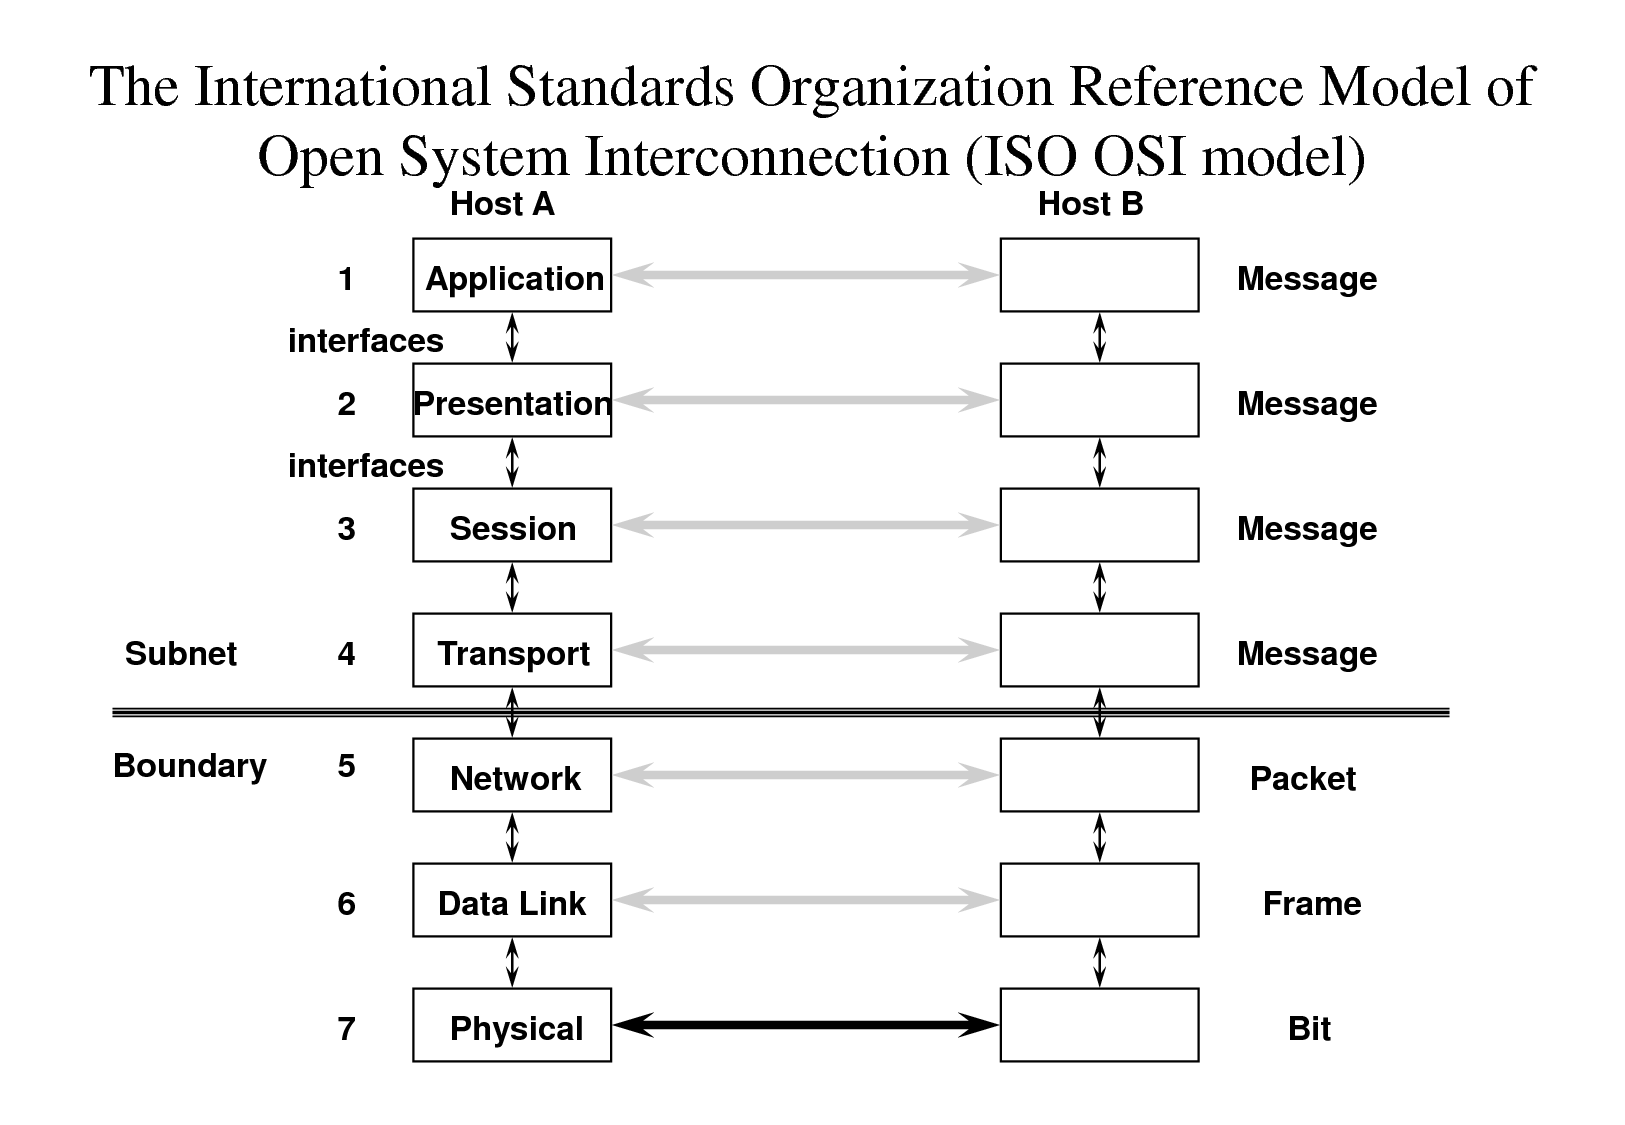
\includegraphics[width=1.\textwidth]{pic/osi.png}
\end{center}
\end{frame}
%--------------------------------------------------------------------------------
\begin{frame}
\small
\begin{itemize}
 \item[N] Физический уровень -- способы трансляции битов в \emph{символы} и их передача в канале связи
 \item[N] Канальный уровень -- организация доступа к среде, исправление ошибок передачи данных
 \item[N] Сетевой уровень -- задачи маршрутизации и обеспечения качества обслуживания
 \item[H] Транспортный уровень -- контроль за потоком передачи данных
 \item[H] Сеансовый уровень -- организация сеансов связи (SIP, RTP)
 \item[H] Уровень представления -- переработка передаваемых данных из потока байтов в пользовательские структуры данных
 \item[H] Прикладной уровень -- набор протоколов, необходимый пользователям (HTTP)
\end{itemize}
N -- Сетевое взаимодействие.
H -- протоколы, выполняемые на хостах.
\end{frame}
%--------------------------------------------------------------------------------
\begin{frame}
 \frametitle{Инкапсуляция}
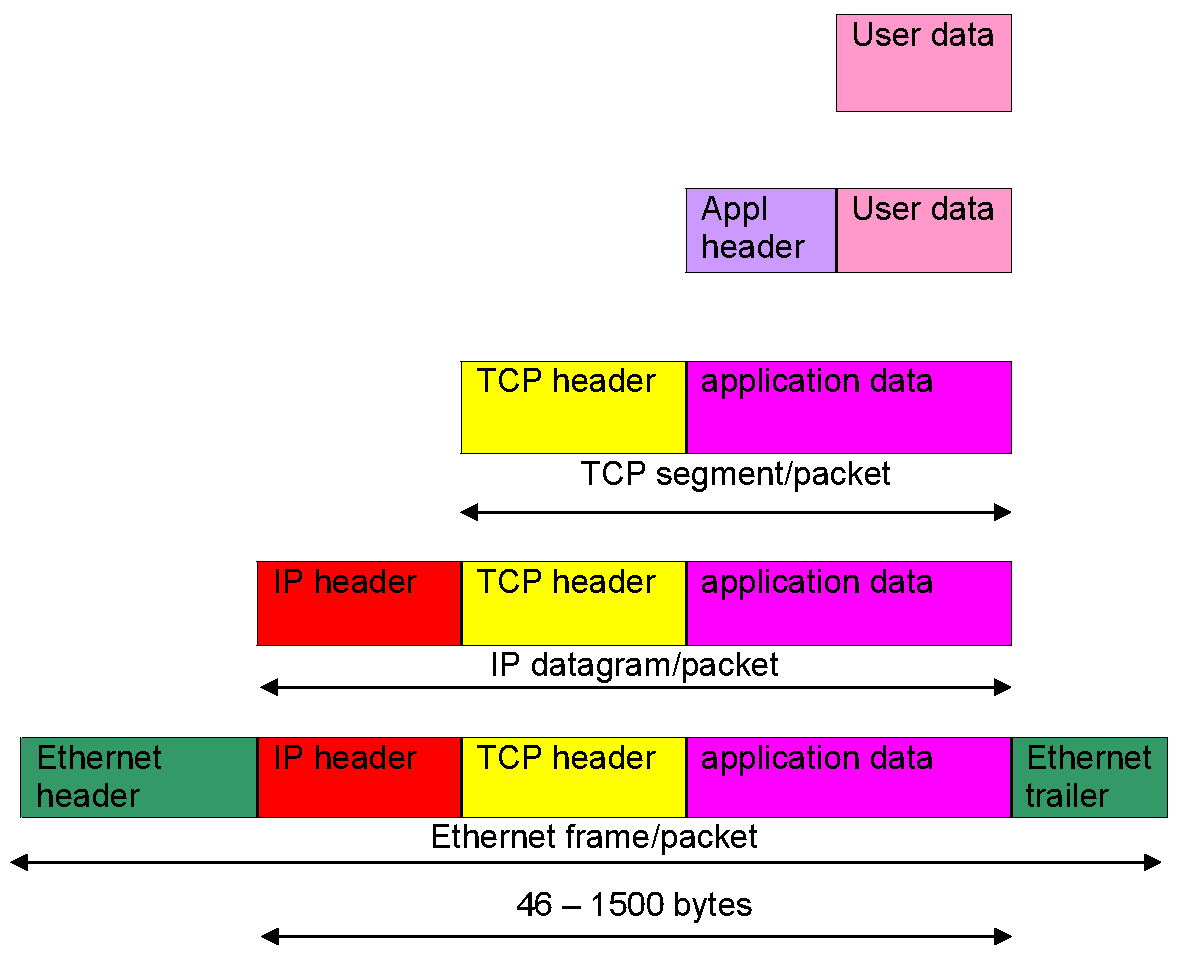
\includegraphics[width=0.8\textwidth]{pic/Encapsulation.png}
\end{frame}
%--------------------------------------------------------------------------------
\section{Эталонная модель TCP/IP}
\begin{frame}
\begin{columns}
\column{.4\textwidth}
\begin{block}{}
\centering
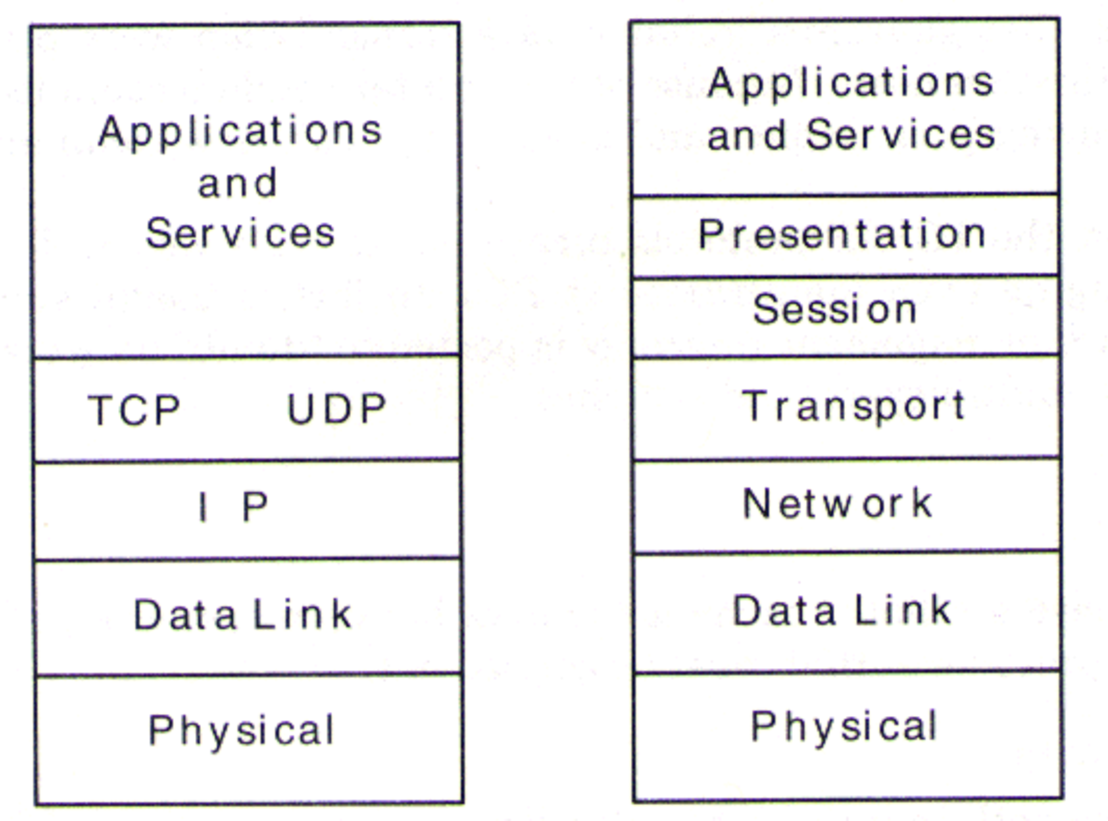
\includegraphics[width=1.2\textwidth]{pic/tcpip.pdf}
\end{block}
\column{.6\textwidth}
\begin{block}{TCP/IP by ARPANET}
\begin{itemize}
        \item Интернет уровень и протокол IP -- основа \emph{коммутации пакетов}
        \item Транспортный уровень -- надёжный поток байт (установление соединения) и дейтаграммный сервис (без установления соединения)
        \item Все остальное -- прикладной уровень (пространство пользователя в OS Linux)
\end{itemize}
\end{block}
\end{columns}
\frametitle{Альтернатива эталонной модели OSI}
\end{frame}
%--------------------------------------------------------------------------------
\begin{frame}
\begin{block}{Концепции модели OSI}
\begin{itemize}
	\item[$+$]Службы. Интерфейсы. Протоколы. Идеальное соответствие идеям ООП.
	\item [$+$] Разработка архитектуры до появления протоколов
	\item [$-$] Отсутствие у разработчиков опыта построения реальных сетей: широковещание не вписывается в данную архитектуру
	\item[$-$] Неявное предположение о жёсткой стандартизации
\end{itemize}
\end{block}
\begin{block}{От протоколов к модели: TCP/IP}
\begin{itemize}
	\item[$+$]Сетевой уровень -- только не ориентированные на соединение сервисы
	\item[$-$]Отсутствие концепции ``Интерфейс-Сервис-Протокол''
\end{itemize}
\end{block}
\end{frame}
%--------------------------------------------------------------------------------
\section{Примеры компьютерных сетей}
%--------------------------------------------------------------------------------
\begin{frame}
\frametitle{ARPANET -- от телефонной сети к распределённой (195х)}
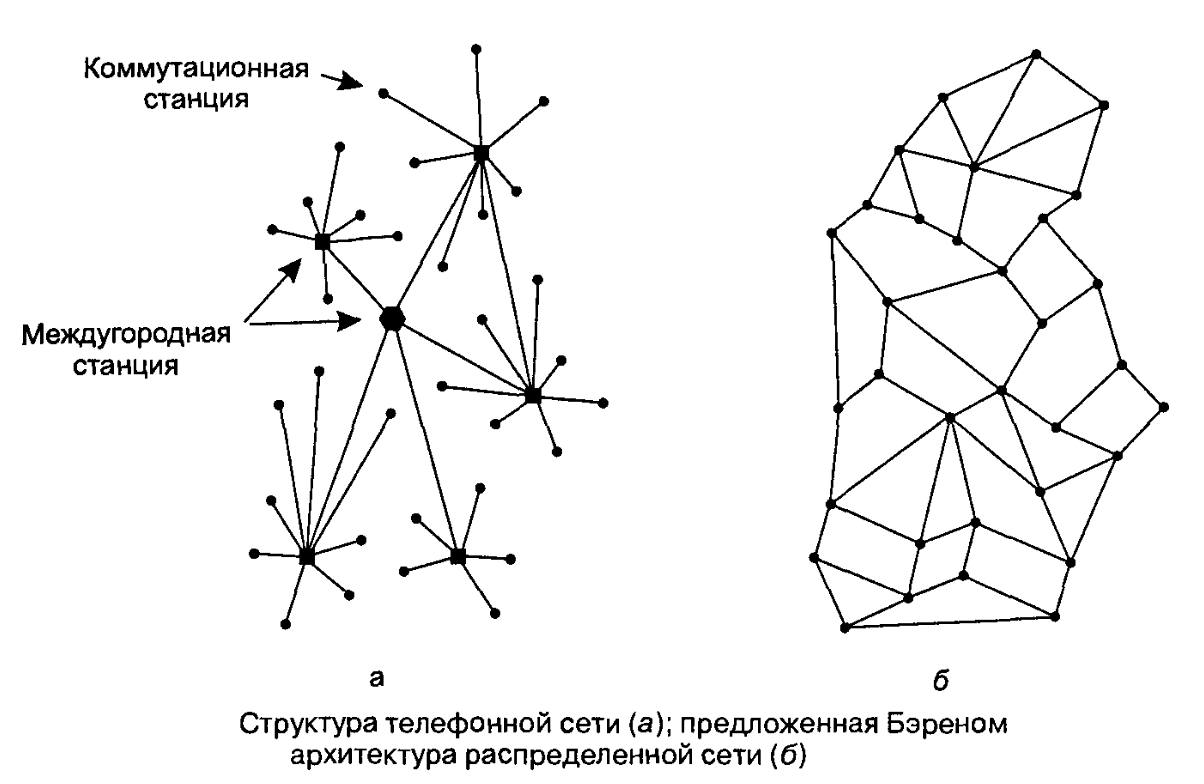
\includegraphics[width=\textwidth]{pic/arpanet.png}
\end{frame}
%--------------------------------------------------------------------------------
\begin{frame}
\frametitle{ARPANET -- передача цифровых данных в распределённой сети}
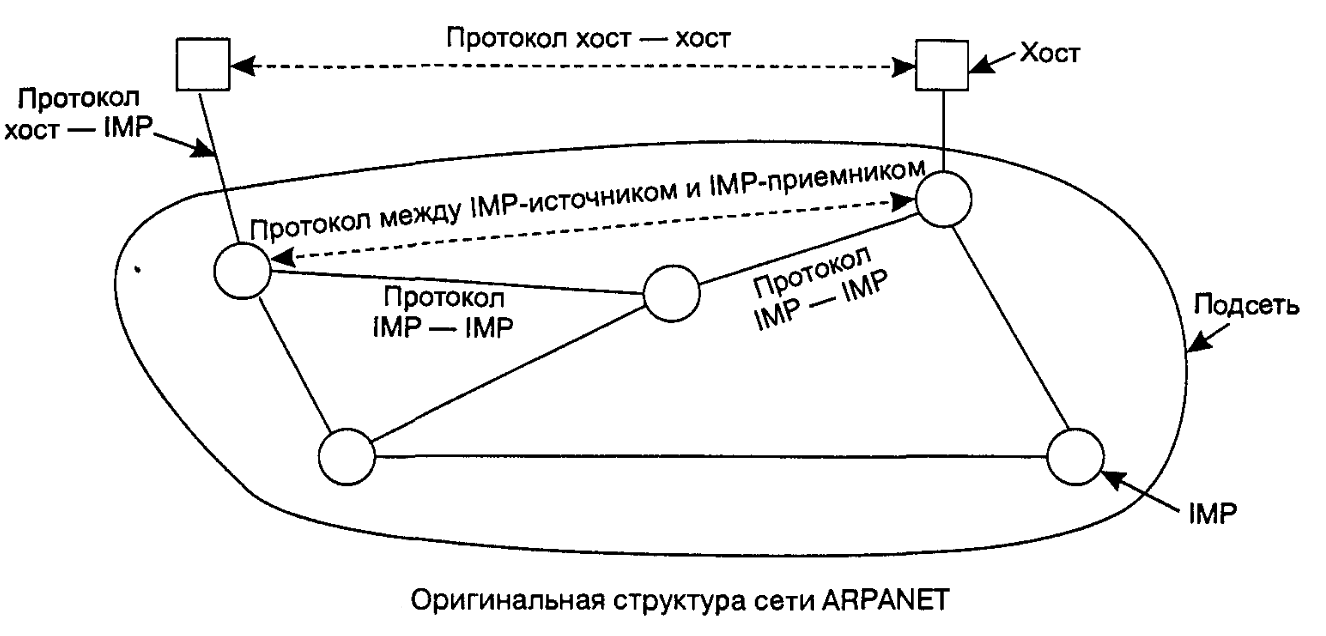
\includegraphics[width=\textwidth]{pic/arpanet-original.png}
\newline
IMP -- Interface Message Processor. Линии связи 56 Кбит/с. Сеть с коммутацией пакетов и промежуточным хранением.
\end{frame}
%--------------------------------------------------------------------------------
\begin{frame}
\frametitle{ARPANET --от 1969 до 1972 годов}
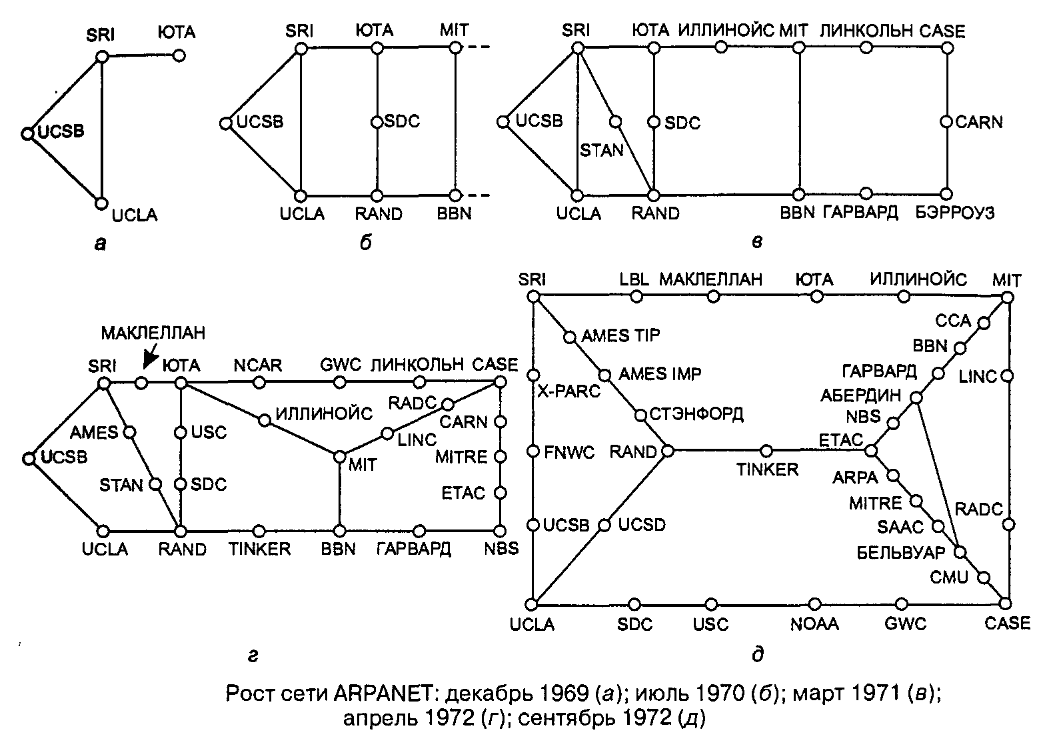
\includegraphics[width=0.93\textwidth]{pic/arpanet-development.png}
\newline
\end{frame}
%--------------------------------------------------------------------------------
\begin{frame}
\frametitle{Развитие ARPANET}
\begin{itemize}
	\item Разработка пакетной мобильной сети
	\item Разработка спутниковой сети
\end{itemize}
\begin{description}
\item[Результат:] Необходимость разработки механизмов объединения сетей.
\item[1974:] Изобретение модели протоколов TCP/IP
\end{description}
\end{frame}
%--------------------------------------------------------------------------------
\begin{frame}
\frametitle{Интернет}
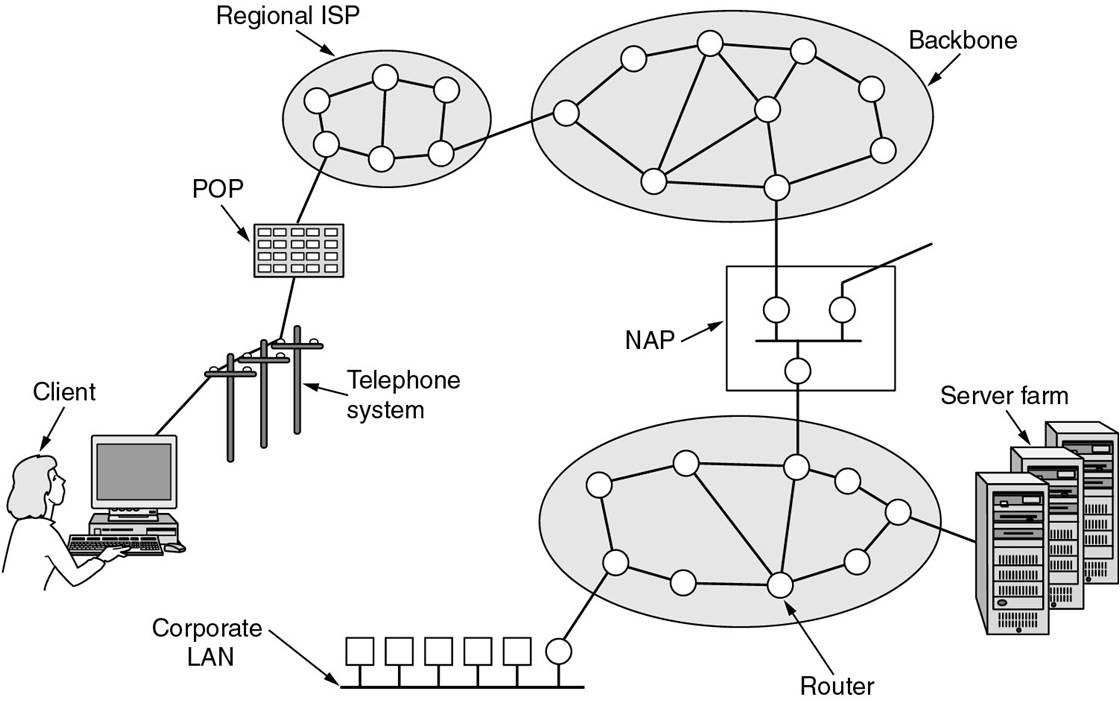
\includegraphics[width=0.93\textwidth]{pic/internet-overview.jpg}
\end{frame}
%--------------------------------------------------------------------------------
\begin{frame}
\frametitle{ATM -- Асинхронный режим передачи}
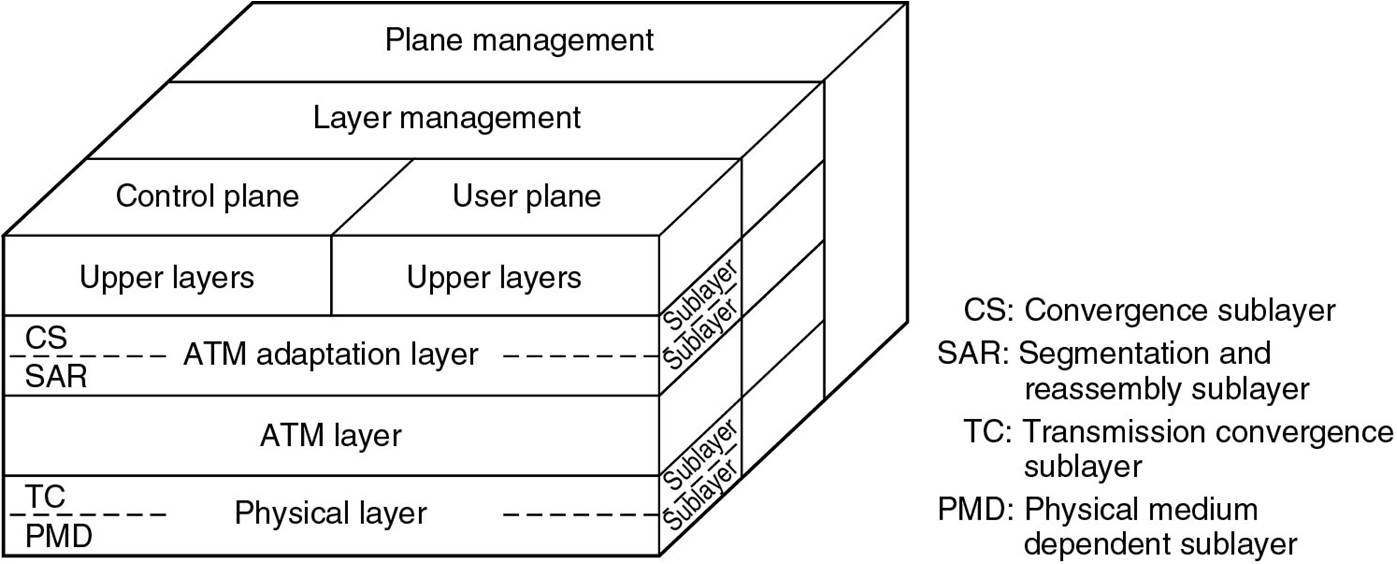
\includegraphics[width=0.93\textwidth]{pic/atm-reference.jpg}
\end{frame}
%--------------------------------------------------------------------------------
\begin{frame}
\frametitle{ATM -- Асинхронный режим передачи}
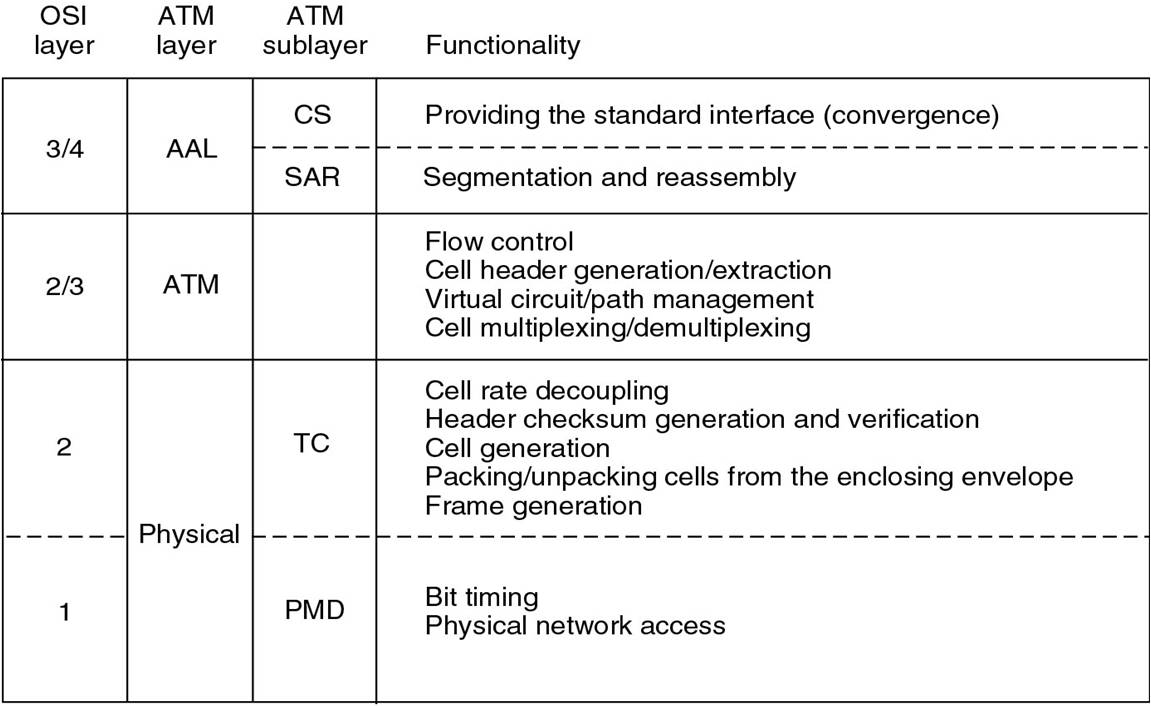
\includegraphics[width=0.93\textwidth]{pic/atm-layers.jpg}
\end{frame}
%--------------------------------------------------------------------------------
\begin{frame}
\frametitle{Особенности беспроводных сетей}
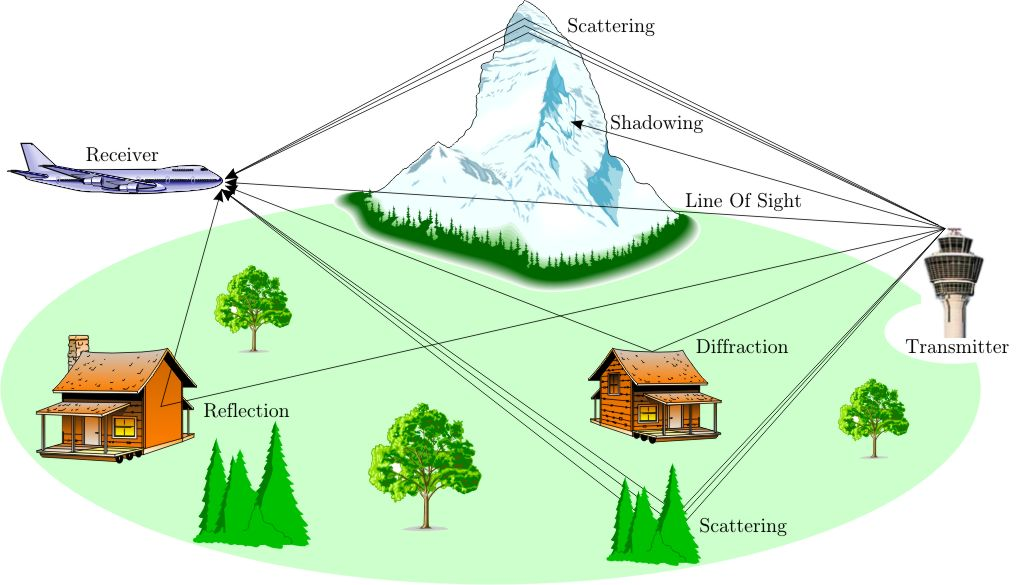
\includegraphics[width=0.93\textwidth]{pic/multipath_propagation.png}
\end{frame}
%--------------------------------------------------------------------------------
\begin{frame}
\frametitle{Архитектура UMTS}
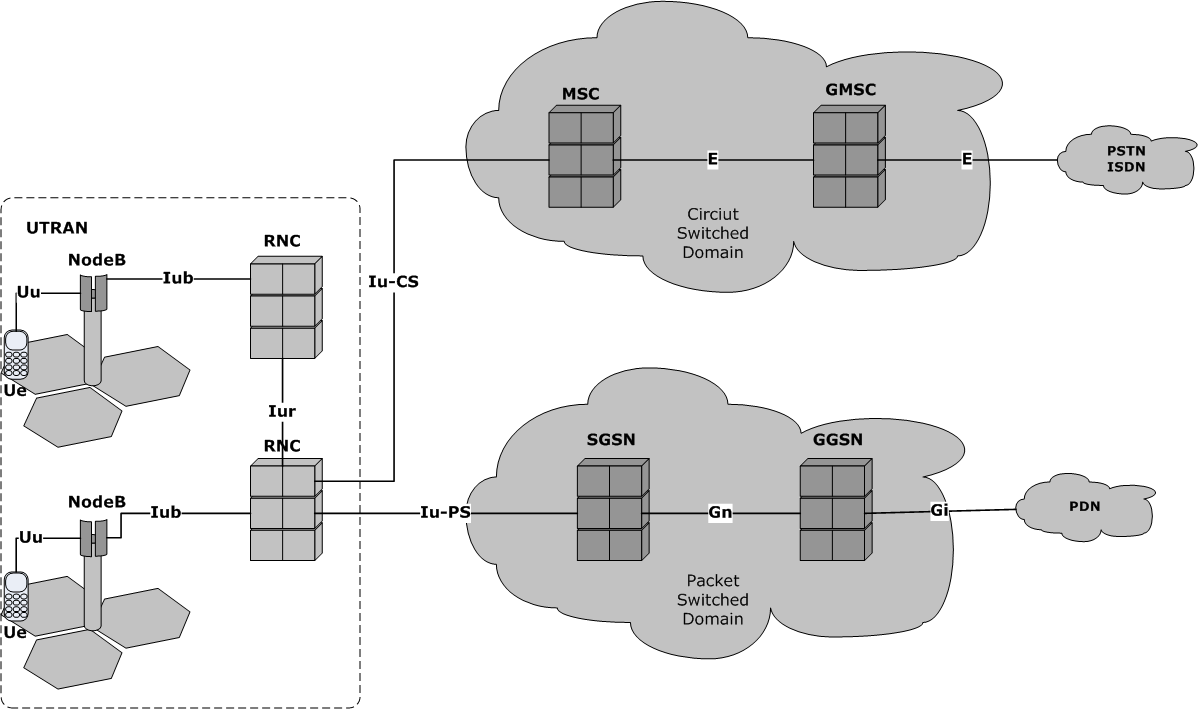
\includegraphics[width=0.93\textwidth]{pic/UmtsArchitecture.png}
\end{frame}
%--------------------------------------------------------------------------------
\end {document}
